\section{Descrição de Software}

O pacote de trabalho de Planejamento e Gerenciamento foi modelado utilizando a notação BPMN, conforme ilustrado na Figura~\ref{fig_bpmn}. A utilização do BPMN permite representar de forma clara e padronizada os processos do projeto, facilitando a compreensão, a análise e a comunicação entre os envolvidos. Por meio desse modelo, é possível visualizar as atividades, os responsáveis, os fluxos de informações e as dependências, contribuindo para uma gestão mais eficiente e alinhada aos objetivos do projeto.

\begin{figure}[H]
\centering
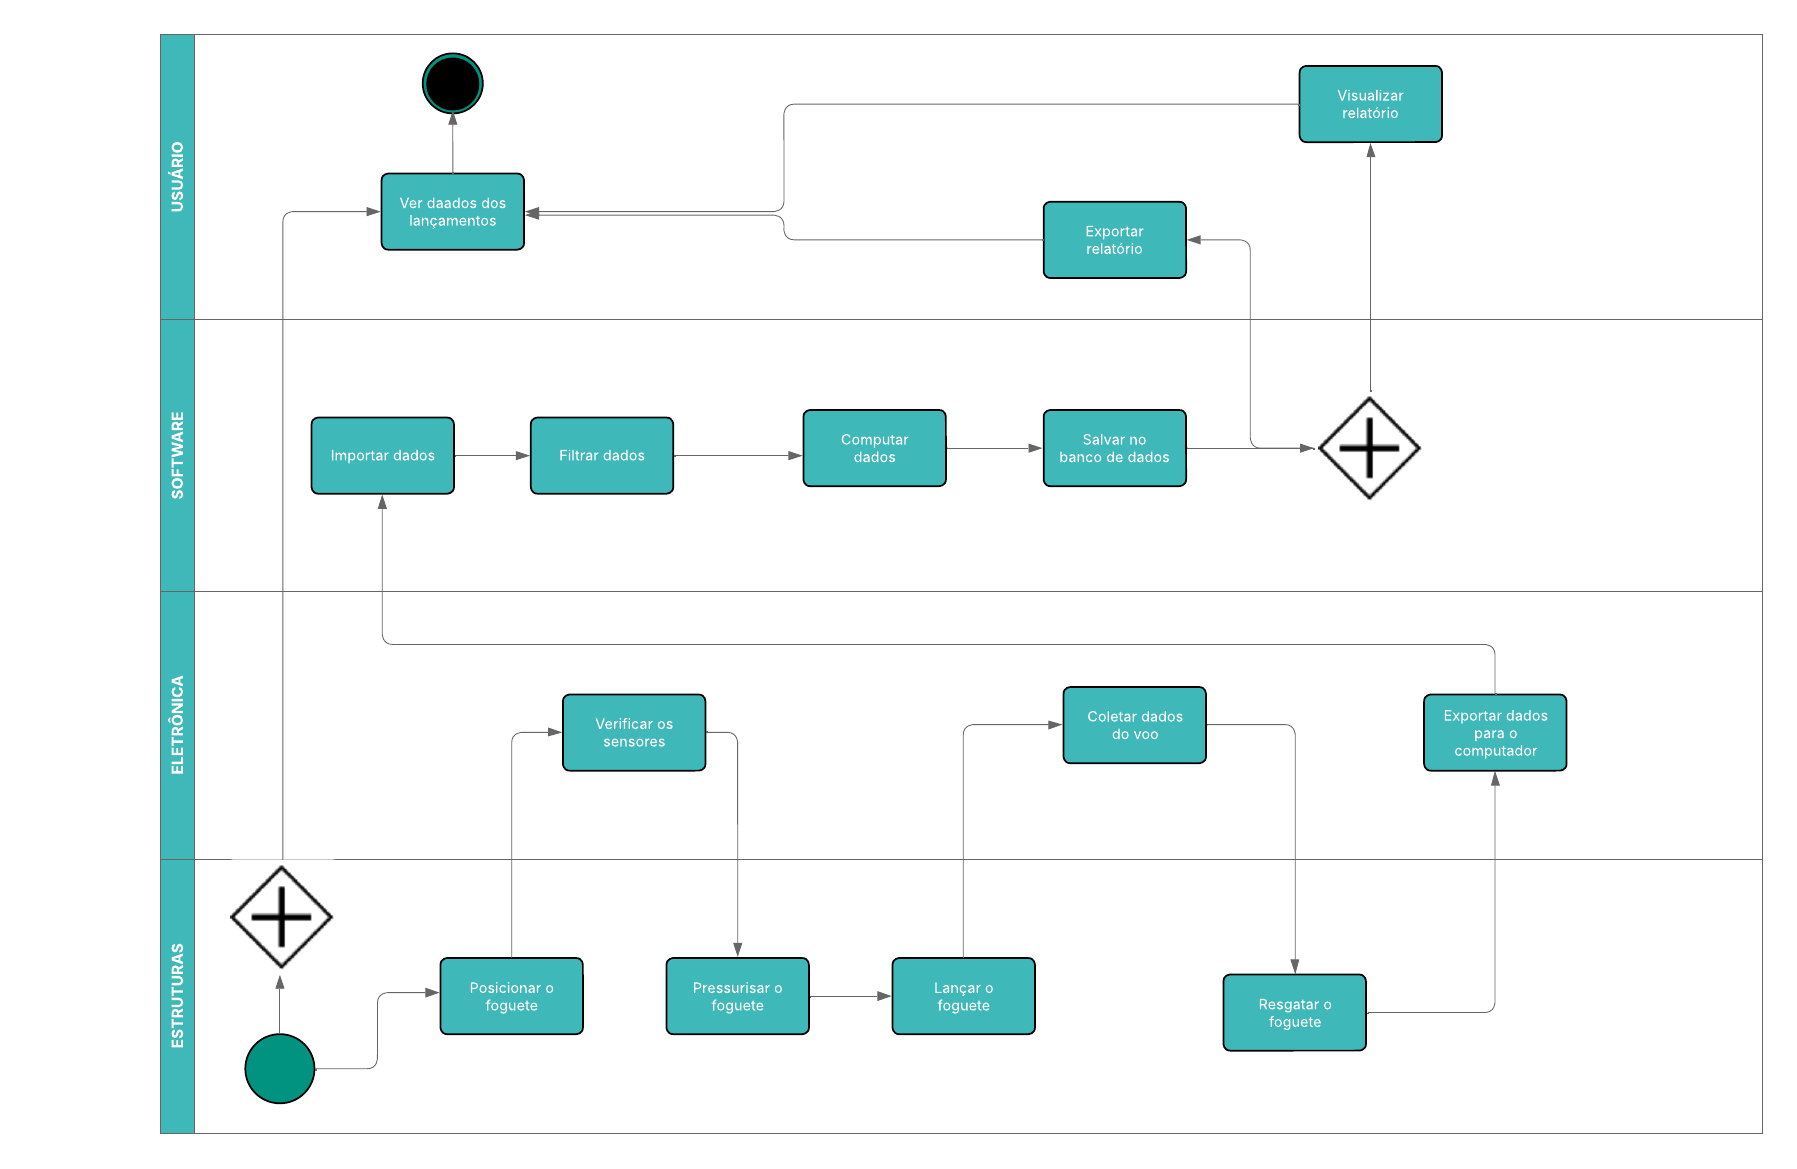
\includegraphics[width=15cm]{figuras/bpmn.png}
\caption{BPMN}
\label{fig_bpmn}
\end{figure}

% -------------------------------------------------------------
% MOSCOW
% -------------------------------------------------------------

\begin{samepage}
O pacote MOSCOW é uma técnica de priorização de requisitos que classifica as funcionalidades em quatro categorias: Must have (deve ter), Should have (deveria ter), Could have (poderia ter) e Won't have this time (não terá desta vez). Essa abordagem ajuda a focar no que é essencial para o sucesso do projeto, garantindo que os recursos sejam alocados de forma eficiente. A Figura \ref{tab:requisitos_projeto} ilustra a aplicação dessa técnica no contexto do projeto.

\begin{landscape}

\begin{figure}[H]
\centering
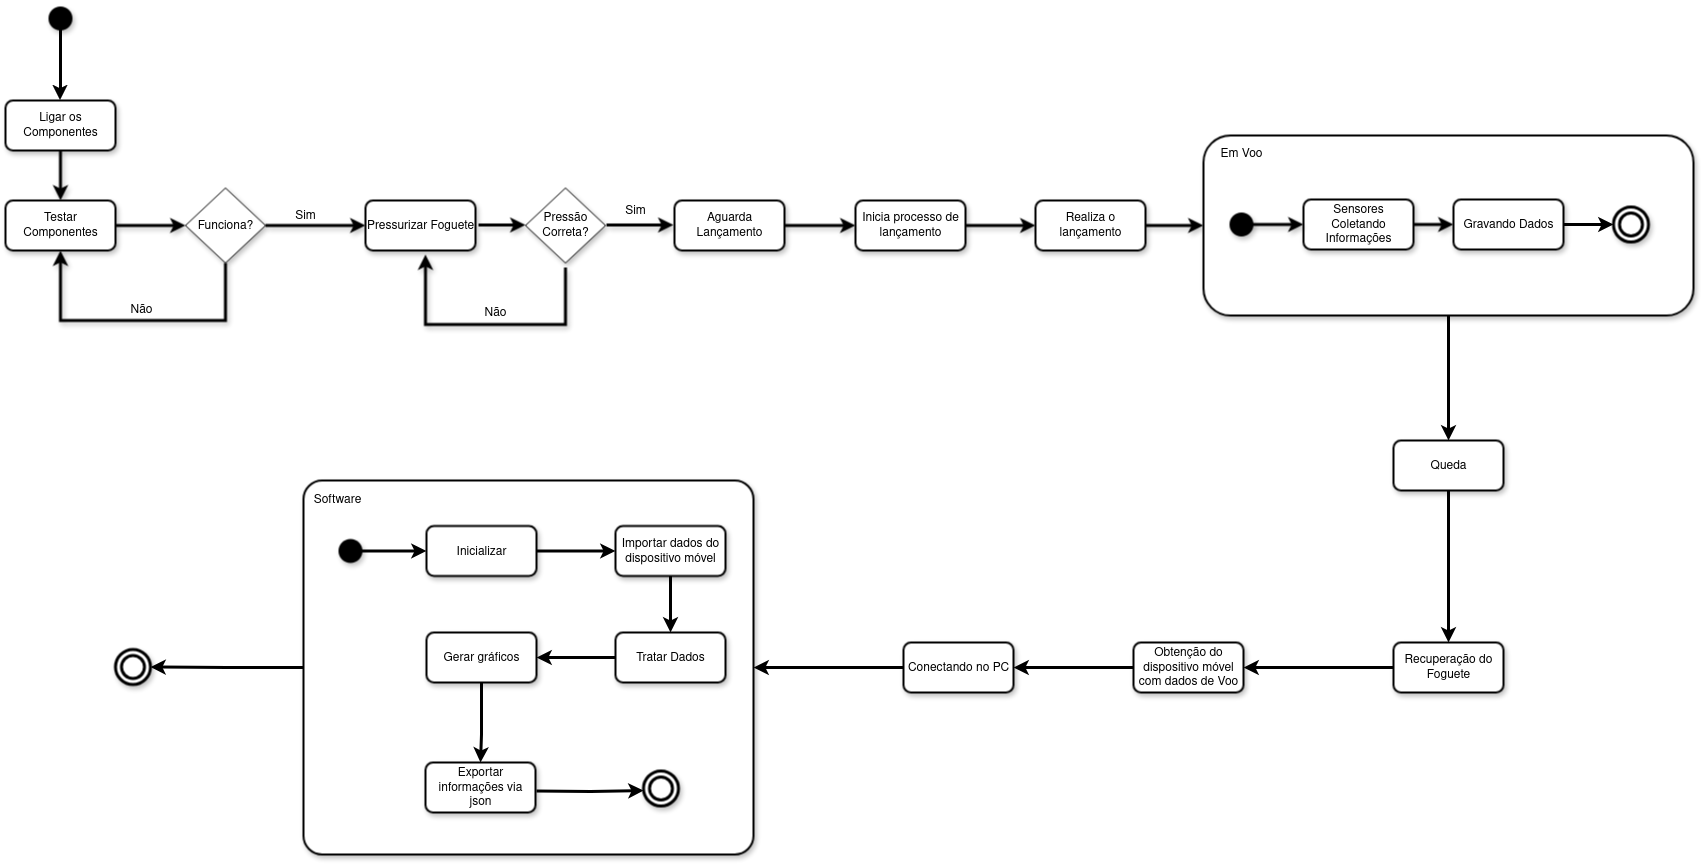
\includegraphics[width=\linewidth,keepaspectratio]{figuras/diagrama_de_estados.png}
\caption{Diagrama de Estados}
\label{fig_diagrama_estados}
\end{figure}

\end{landscape}


\begin{table}[H]
\centering
\scriptsize
\setlength{\tabcolsep}{4pt}
\caption{Tabela de Requisitos do Projeto}
\begin{tabular}{|l|p{8cm}|l|}
\hline
Id. & Descição & Prioridade \\
\hline
RQ01 & Importar dados de voo em JSON de dispositivo externo & Must have \\
\hline
RQ02 & Exibir gráfico de velocidade vertical vs. tempo. & Must have \\
\hline
RQ03 & Exibir gráfico de aceleração vertical vs. tempo. & Must have \\
\hline
RQ04 & Exibir gráfico de dispersão da trajetória no plano X e Y. & Must have \\
\hline
RQ05 & Exibir gráfico de altitude vs. tempo. & Must have \\
\hline
RQ06 & Exibir valores máximos e mínimos de aceleração, velocidade e ângulo. & Should have \\
\hline
RQ07 & Exibir tempo de execução e intervalos de amostragem. & Should have \\
\hline
RQ08 & Exportar dados do voo em JSON. & Must have \\
\hline
RQ09 & Importar arquivos JSON para comparação e simulação. & Must have \\
\hline
RQ10 & Aplicar filtro de média móvel nos dados dos sensores. & Should have \\
\hline
RQ11 & Inicializar o sistema de medição e sinalizar prontidão para o lançamento. & Must Have \\
\hline
RQ12 & Aplicar filtro de média móvel nos dados dos sensores. & Must Have \\
\hline
RQ13 & O mecanismo de lançamento deve permitir disparo seguro por tração de corda a pelo menos 5 metros. & Must Have \\
\hline
RQ14 & A plataforma de lançamento deve manter o foguete estável até o momento da liberação manual. & Must Have \\
\hline
\end{tabular}
\label{tab:requisitos_projeto}
\end{table}

\end{samepage}


% -------------------------------------------------------------
% REQUISITOS NÃO-FUNCIONAIS
% -------------------------------------------------------------

\begin{samepage}
Os requisitos não-funcionais são critérios que definem a qualidade e as restrições do sistema, como desempenho, segurança, usabilidade e portabilidade. Eles são essenciais para garantir que o sistema atenda às expectativas dos usuários e funcione de maneira eficiente em diferentes ambientes. A Tabela \ref{tab:requisitos_nao_funcionais} apresenta os requisitos não-funcionais identificados para o projeto.

\begin{table}[H]
\centering
\scriptsize
\setlength{\tabcolsep}{4pt}
\caption{Requisitos Não-Funcionais}
\begin{tabular}{|l|p{11cm}|}
\hline
Id. & Descrição \\
\hline
RNF01 & Os dados dos lançamentos devem ser armazenados localmente de forma que não possam ser corrompidos em caso de desligamento inesperado. \\
\hline
RNF02 & O software deve validar a integridade dos arquivos JSON antes de processar os dados. \\
\hline
RNF03 & O software deve ser multiplataforma, funcionando em pelo menos Windows, Linux e MacOS. \\
\hline
RNF04 & Não deve depender de conexão com internet para funcionar. \\
\hline
RNF05 & A geração de relatórios e gráficos não deve exceder 3 segundos para arquivos de até 100 linhas de dados do lançamento. \\
\hline
RNF06 & A interface gráfica (GUI) deve ser intuitiva, com botões claros para importar dados, gerar gráficos e acessar os lançamentos anteriores. \\
\hline
RNF07 & A interface de linha de comando (CLI – Command Line Interface) deve oferecer comandos simples para uso técnico ou automatizado. \\
\hline
\end{tabular}
\label{tab:requisitos_nao_funcionais}
\end{table}
\end{samepage}

% -------------------------------------------------------------
% CASOS DE USO
% -------------------------------------------------------------

\begin{samepage}

O pacote de Casos de Uso é uma técnica de modelagem que descreve as interações entre os usuários (atores) e o sistema, detalhando como os requisitos funcionais serão atendidos. Os casos de uso ajudam a identificar as funcionalidades essenciais do sistema e a garantir que todas as partes interessadas tenham uma compreensão clara dos objetivos do projeto. A Figura \ref{fig_casos_de_uso} apresenta um exemplo de diagrama de casos de uso utilizado no projeto.
\begin{figure}[H]
	\centering
	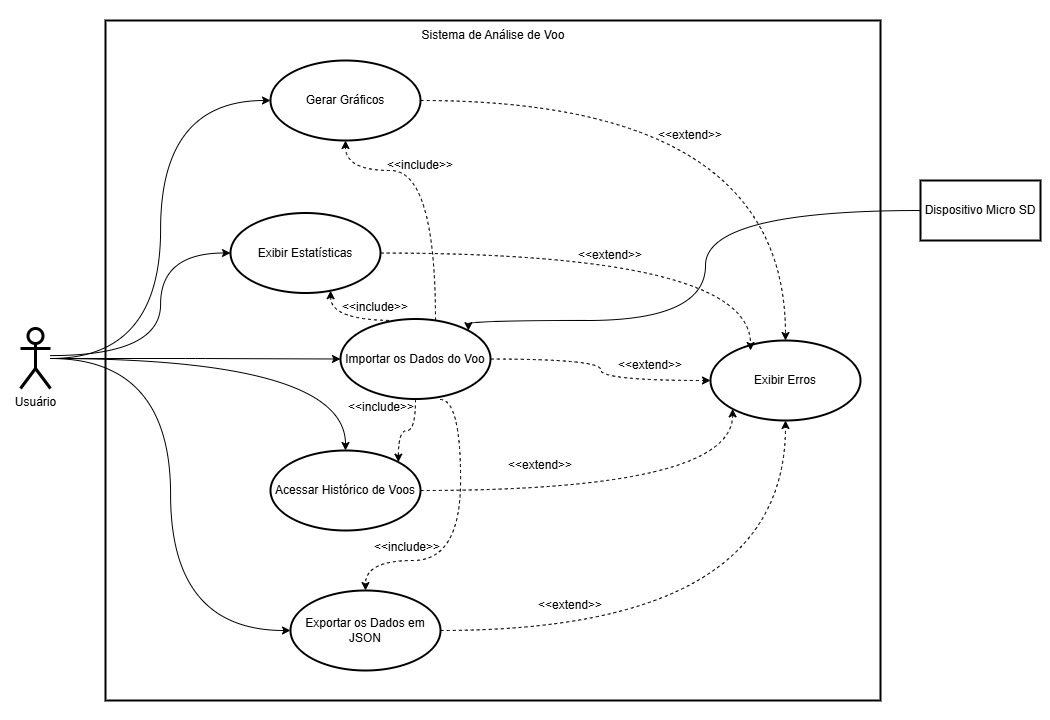
\includegraphics[width=15cm]{figuras/caso_de_uso.png}
	\caption{Casos de Uso}
	\label{fig_casos_de_uso}
\end{figure}
\end{samepage}

% -------------------------------------------------------------
% DIAGRAMA DE ENTIDADE-RELACIONAMENTO
% -------------------------------------------------------------

\begin{samepage}

O Diagrama de Entidade-Relacionamento (DER) é uma técnica de modelagem de dados que representa as entidades do sistema e os relacionamentos entre elas. É fundamental para a construção do banco de dados e para garantir que os dados sejam organizados de forma eficiente. A Figura \ref{fig_der} ilustra um exemplo de DER utilizado no projeto.

\begin{figure}[H]
	\centering
	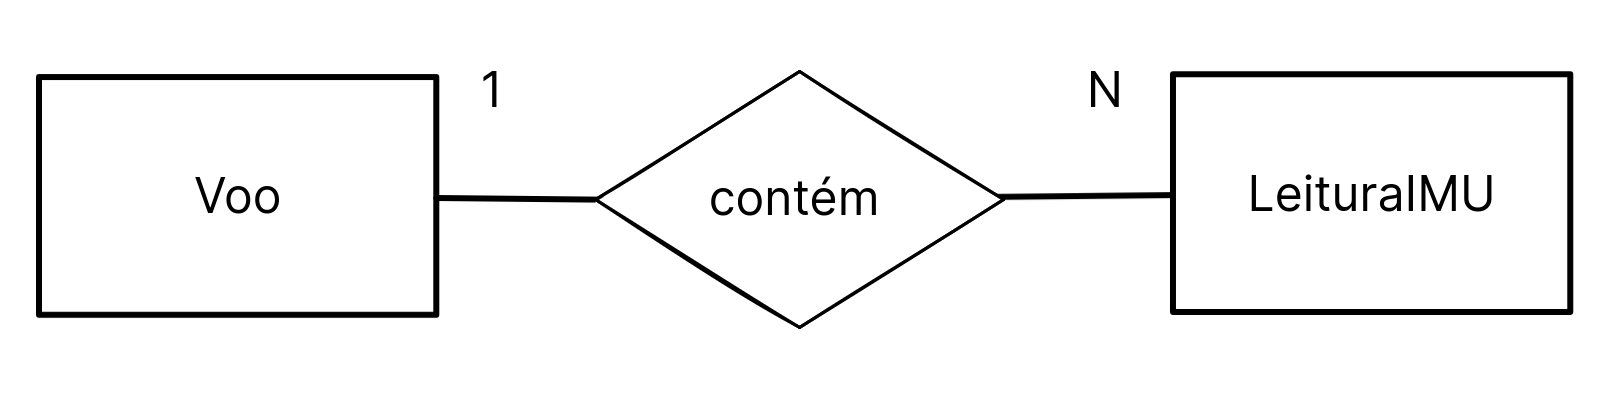
\includegraphics[width=15cm]{figuras/der.png}
	\caption{Diagrama de Entidade-Relacionamento}
	\label{fig_der}
\end{figure}

Após isso, podemos modelar os atributos de cada entidade, conforme os dados que receberemos da ERP32, que calculará movimentos de unidade de medição inercial pelo sensor de 6 eixos, como o acelerômetro e o giroscópio. A Figura \ref{fig_atributos} apresenta um exemplo de atributos modelados para as entidades do sistema.

\begin{figure}[H]
	\centering
	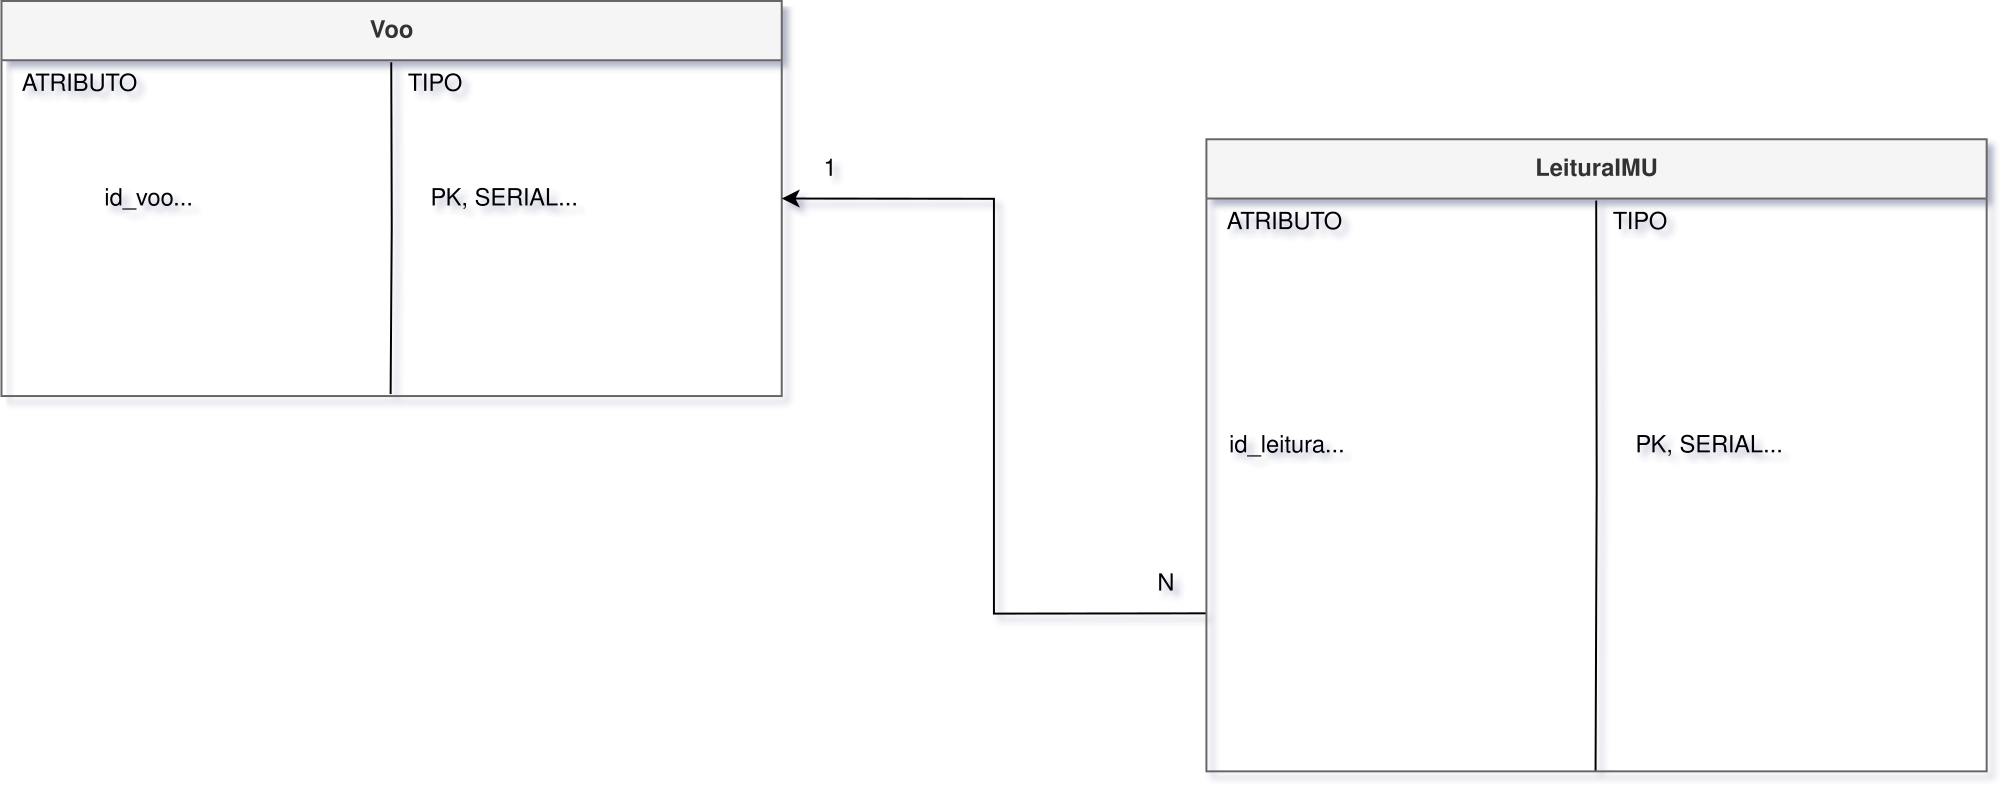
\includegraphics[width=15cm]{figuras/atributos.png}
	\caption{Atributos das Entidades}
	\label{fig_atributos}
\end{figure}

\end{samepage}

% -------------------------------------------------------------
% ARQUITETURA DO SOFTWARE
% -------------------------------------------------------------

\begin{samepage}

O padrão arquitetural escolhido é o Monolítico, por se tratar de um sistema simples, com poucos módulos e baixa complexidade. A adoção de uma arquitetura mais robusta, como microsserviços, não se justifica neste contexto, uma vez que todo o processamento ocorre localmente e o software não possui dependências distribuídas. 

A arquitetura monolítica permite concentrar todas as funcionalidades como leitura de dados, processamento, geração de relatórios e apresentação dos resultados em um único sistema, facilitando o desenvolvimento, testes e manutenção dentro dos requisitos do projeto, como visto na Figura \ref{fig_arquitetura}.

\begin{figure}[H]
	\centering
	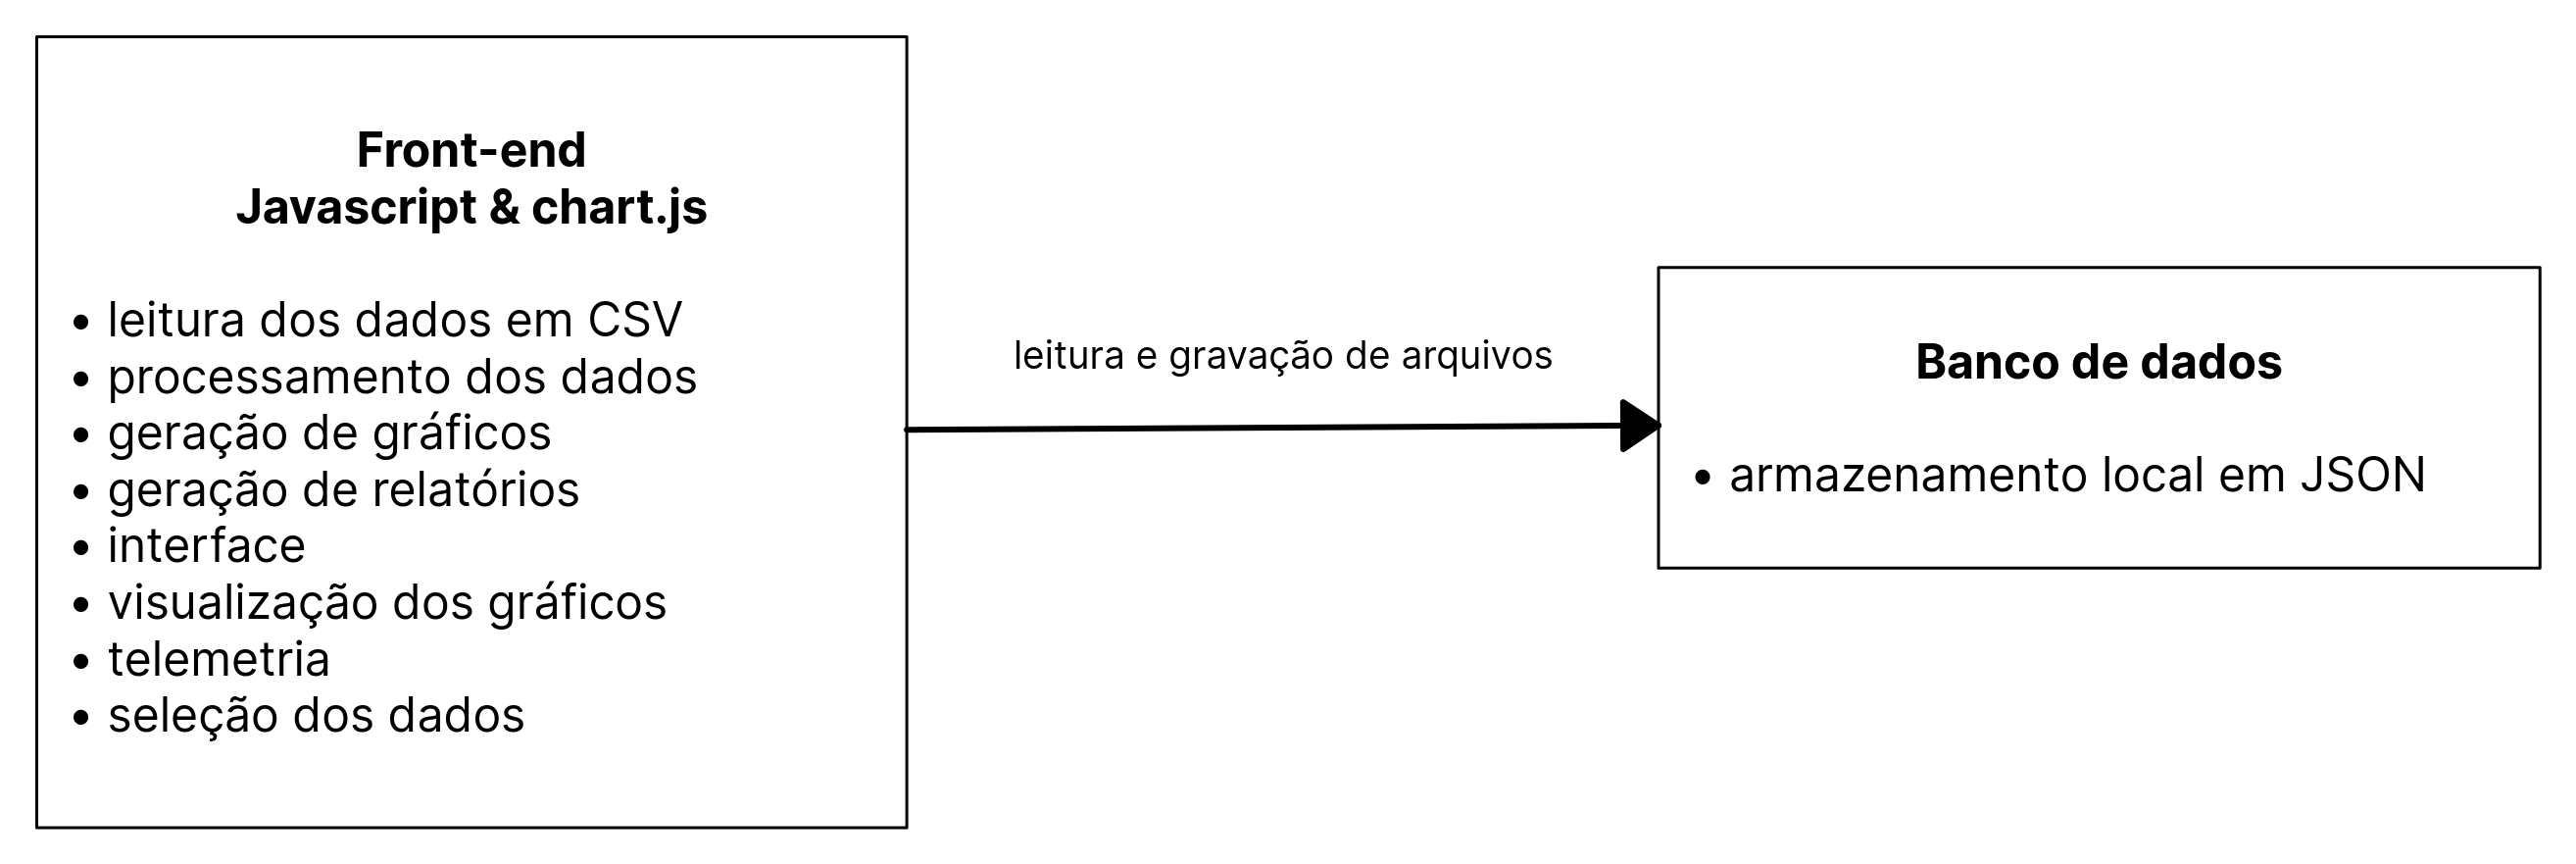
\includegraphics[width=0.75\textwidth,height=0.5\textheight,keepaspectratio]{figuras/arquitetura2.png}
	\caption{Arquitetura do Software}
	\label{fig_arquitetura}
\end{figure}

As linguagens de programação escolhidas para o desenvolvimento do software são Python e JavaScript, cada uma com suas responsabilidades específicas dentro do sistema.

Python foi responsável primariamente pelo desenvolvimento de uma interface de linha de comando (CLI). Utilizado para processamento dos dados, geração de relatórios, análises estatísticas e manipulação dos arquivos JSON até a segunda entrega. Utilizamos as bibliotecas Pandas para manipulação e análise de dados. NumPy para cálculos matemáticos e operações com arrays. E Matplotlib para criação de gráficos e visualizações dos dados.

JavaScript então foi utilizado no desenvolvimento do frontend (GUI), através da biblioteca Chart.JS, para então cumprir com as responsabilidades do CLI, e apresentando visualmente os dados dos lançamentos de forma interativa e amigável.

Neste projeto, não foi utilizado um banco de dados tradicional. Os dados dos lançamentos são armazenados localmente em arquivos JSON, por se tratar de uma solução leve, simples e suficiente para o volume de dados do projeto. Cada arquivo JSON conterá os dados de um lançamento específico, organizados de forma que possam ser facilmente acessados tanto pela CLI quanto pela interface gráfica.

\end{samepage}

% -------------------------------------------------------------
% PROTÓTIPO
% -------------------------------------------------------------

\begin{samepage}

O protótipo do software foi desenvolvido utilizando a ferramenta Figma, que permite criar interfaces interativas e de alta fidelidade. O protótipo inclui telas para importação de dados, visualização de gráficos, relatórios e histórico de lançamentos. Ele pode ser acessado em \href{https://www.figma.com/proto/hpceGFGo6mcwMjRJsKIyG7/Foguete-D-agua?node-id=19-2848&p=f&t=BINV4uEIBSLAGqsi-1&scaling=min-zoom&content-scaling=fixed&page-id=0%3A1&starting-point-node-id=19%3A2848}{neste endereço}.

\end{samepage}

% -------------------------------------------------------------
% MODIFICAR PARA EXPLICART OS TESTES DO PROJETO	
% -------------------------------------------------------------

\begin{samepage}

A principal mudança nos testes foi a especificação e detalhamento dos mesmos. Todos os casos de teste foram migrados do relatório para uma planilha no Microsoft Excel Online, como disponibilizado anteriormente, facilitando a visualização geral, o acompanhamento da execução e a atualização dos status de cada teste em tempo real por todos os membros da equipe. Ela pode ser completamente acessada em
\href{https://unbbr.sharepoint.com/:x:/s/PI1-Grupo2330/EY-ZE1arh2RGgJju4ij_Er4BGhCN5S1qYQiIwdHMMRtLBg?e=fs9Vxi}{planilha de testes do grupo 2}.

% Para o caso de teste CT01, que envolve a importação de um arquivo JSON válido, foi adicionado um exemplo de arquivo JSON com dados reais do foguete. Esse arquivo contém informações como id do voo, tempo, aceleração e velocidade, permitindo uma validação mais precisa do processo de importação. No mesmo contexto, ao CT02 foi adicionado um arquivo JSON com campos ausentes, como id de leitura e tempo, para testar a robustez do sistema em lidar com dados incompletos. O CT03 foi modificado para incluir um arquivo JSON com formato inválido, como strings onde se esperavam números, para verificar a capacidade do sistema de identificar e reportar erros de formatação.

\subsection{Testes}

Aos testes CT01, CT02, CT03, CT08, CT11, CT13, CT14, CT15, CT16 foram adicionados os dados de arquivo necessário para realização do teste, a estrutura dos dados de entrada, especificação de resultados esperados e, para os que possui mensagens, as de sucesso e erro foram definidas. Para o teste de responsividade (CT05) foram definidos os tamanhos da tela para responsividade. 

Na parte de hardware, houve modificações significativas. Para o CT06, os dados agora são feitos de forma analógica usando um barômetro.  Para CT22, agora o atuador é o manômetro; para CT24, a conectividade agora é feita com cartão SD e ambos os testes foram reelaborados. Os testes CT17, CT19 e CT21 foram eliminados por conta de mudanças realizadas no hardware. 

Sobre estruturas, no CT07, foi definido a quantidade de água a ser utilizada no teste.  Os testes não citados foram mantidos da mesma forma, pois não foi observado uma necessidade de alteração. 

\subsection{Resultados}

Para os voos administrados no dia de apresentação do projeto, foram realizados três lançamentos com o foguete, e seus dados foram coletados e armazenados em arquivos CSV, por conta de ruídos e interferências, os dados foram filtrados e processados para garantir a precisão dos resultados. Esses dados estão disponíveis no repositório do projeto, permitindo a análise e validação dos resultados obtidos durante os testes, que podem ser acessados no \href{https://github.com/melohugo/PI1}{repositório do projeto}. Note que o tempo é acumulado pelos voos anteriores, para que assim possa se ver os três voos em conjunto. Segue então os gráficos gerados a partir desses mesmos dados:

\begin{landscape}

\begin{figure}[H]
\centering
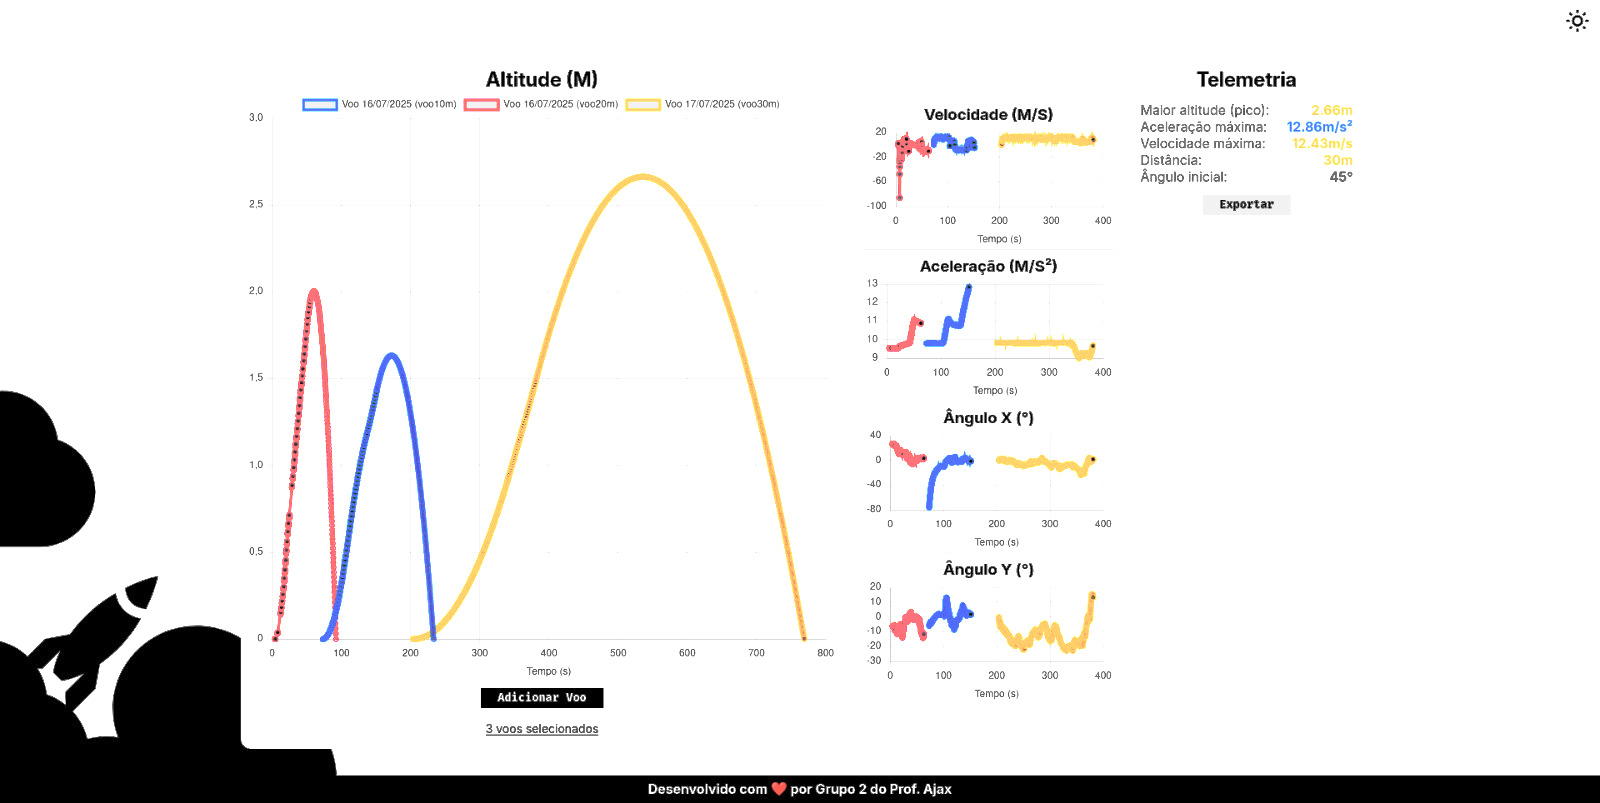
\includegraphics[width=\linewidth,keepaspectratio]{figuras/software/graficos.jpeg}
\caption{Gráficos de desempenho dos voos.}
\label{fig_graficos}
\end{figure}

\end{landscape}

\end{samepage}
% \include{editaveis/secoes/testes}